\documentclass[a4paper]{scrreprt}

% Uncomment to optimize for double-sided printing.
% \KOMAoptions{twoside}

% Set binding correction manually, if known.
% \KOMAoptions{BCOR=2cm}

% Localization options
\usepackage[english]{babel}
\usepackage[T1]{fontenc}
\usepackage[utf8]{inputenc}

% Quotations
\usepackage{dirtytalk}

% Floats
\usepackage{float}

\usepackage{numbertabbing}

% Enhanced verbatim sections. We're mainly interested in
% \verbatiminput though.
\usepackage{verbatim}

% Automatically remove leading whitespace in lstlisting
\usepackage{lstautogobble}

% PDF-compatible landscape mode.
% Makes PDF viewers show the page rotated by 90°.
\usepackage{pdflscape}

% Advanced tables
\usepackage{array}
\usepackage{tabularx}
\usepackage{longtable}

% Fancy tablerules
\usepackage{booktabs}

% Graphics
\usepackage{graphicx}

% Current time
\usepackage[useregional=numeric]{datetime2}

% Float barriers.
% Automatically add a FloatBarrier to each \section
\usepackage[section]{placeins}

% Custom header and footer
\usepackage{fancyhdr}

\usepackage{geometry}
\usepackage{layout}

% Math tools
\usepackage{mathtools}
% Math symbols
\usepackage{amsmath,amsfonts,amssymb}
\usepackage{amsthm}
% General symbols
\usepackage{stmaryrd}

\DeclarePairedDelimiter\abs{\lvert}{\rvert}

% Indistinguishable operator (three stacked tildes)
\newcommand*{\diffeo}{% 
  \mathrel{\vcenter{\offinterlineskip
  \hbox{$\sim$}\vskip-.35ex\hbox{$\sim$}\vskip-.35ex\hbox{$\sim$}}}}

% Bullet point
\newcommand{\tabitem}{~~\llap{\textbullet}~~}

\floatstyle{ruled}
\newfloat{algo}{htbp}{algo}
\floatname{algo}{Algorithm}
% For use in algorithms
\newcommand{\str}[1]{\textsc{#1}}
\newcommand{\var}[1]{\textit{#1}}
\newcommand{\op}[1]{\textsl{#1}}

\pagestyle{plain}
% \fancyhf{}
% \lhead{}
% \lfoot{}
% \rfoot{}
% 
% Source code & highlighting
\usepackage{listings}

% SI units
\usepackage[binary-units=true]{siunitx}
\DeclareSIUnit\cycles{cycles}

% Convenience commands
\newcommand{\mailsubject}{41106 - Cryptography Protocols - Series 2}
\newcommand{\maillink}[1]{\href{mailto:#1?subject=\mailsubject}
                               {#1}}

% Should use this command wherever the print date is mentioned.
\newcommand{\printdate}{\today}

\subject{41106 - Cryptographic Protocols}
\title{Series 2}

\author{Michael Senn \maillink{michael.senn@students.unibe.ch} - 16-126-880}

\date{\printdate}

% Needs to be the last command in the preamble, for one reason or
% another. 
\usepackage{hyperref}

\begin{document}
\maketitle


\setcounter{chapter}{1}

\chapter{Series 2}

\section{Cricuit for comparing two numbers}

\subsection{Algorithm}

Consider the following algorithm for comparing two numbers.

\begin{algo}
  \vbox{
    \small
    \begin{numbertabbing}
      xxxx\=xxxx\=xxxx\=xxxx\=xxxx\=xxxx\=MMMMMMMMMMMMMMMMMMM\=\kill
      \textbf{Input} \\
	  \> Big-endian number $x$: $x_{n-1} \ldots x_0$ \\
	  \> Big-endian number $y$: $y_{n-1} \ldots y_0$ \\
      \textbf{Algorithm} \\
	  \> \var{i} := n \\
	  \> \textbf{while} $i > 0$: \\
	  \> \> \var{i} := \var{i - 1} \\
	  \> \> \textbf{if} $x_i > y_i$: \\
	  \> \> \> \textbf{return} (1, 0) \\
	  \> \> \textbf{if} $y_i > x_i$: \\
	  \> \> \> \textbf{return} (0, 1) \\
	  \> \textbf{return} (1, 1)
    \end{numbertabbing}
  }
  \caption{bigger(x, y)}
  \label{alg:bigger}
\end{algo}

Let $x_i$, $y_i$ be the i-th bit of the two numbers. Let:
\begin{itemize}
		\item $a_i := x_i \oplus y_i$, $a_i = 1 \Leftrightarrow x_i \neq y_i$
		\item $b_i := a_i \land x_i$, $b_i = 1 \Leftrightarrow x_i > y_i$
		\item $c_i := a_i \land y_i$, $c_i = 1 \Leftrightarrow y_i > x_i$
\end{itemize}

Then, with $k_n, j_n := 0$, let:
\begin{itemize}
		\item $j_i := j_{i+1} \lor d_i$
		\item $k_i := k_{i+1} \lor e_i$
		\item $d_i := b_i \land \neg k_{i+1}$
		\item $e_i := c_i \land \neg j_{i+1}$
\end{itemize}

$d_i$ will be equal to $1$ if $x_i > y_i$ and $x_k \geq y_k \forall k > i$,
that is the i-th digit of $x$ is bigger than the i-th digit of $y$, and no
more-significant digit of $y$ was bigger than its counterpart of $x$. Similarly
for $e_i$.

Then, $(j_0, k_0)$ will be $(1, 0)$ if $x > y$, $(0, 1)$ if $x < y$ and $(0,
0)$ if $x = y$.

Finally, let:
\begin{itemize}
		\item $j := j_0 \lor \neg (j_0 \oplus k_0)$
		\item $k := k_0 \lor \neg (j_0 \oplus k_0)$
\end{itemize}

Then, $(j, k)$ will be as required. This allows rewriting the algorithm as
follows:

\begin{algo}
  \vbox{
    \small
    \begin{numbertabbing}
      xxxx\=xxxx\=xxxx\=xxxx\=xxxx\=xxxx\=MMMMMMMMMMMMMMMMMMM\=\kill
      \textbf{Input} \\
	  \> Big-endian number $x$: $x_{n-1} \ldots x_0$ \\
	  \> Big-endian number $y$: $y_{n-1} \ldots y_0$ \\
      \textbf{Algorithm} \\
	  \> \var{i} := n \\
	  \> \var{$j_n$} := 0 \\
	  \> \var{$k_n$} := 0 \\
	  \> \textbf{while} $i > 0$: \\
	  \> \> \var{i} := \var{i - 1} \\
	  \> \> \var{$a_i$} := \var{$x_i$} XOR \var{$y_i$} \\
	  \> \> \var{$b_i$} := \var{$a_i$} AND \var{$x_i$} \\
	  \> \> \var{$c_i$} := \var{$a_i$} AND \var{$y_i$} \\
	  \\
	  \> \> \var{$d_i$} := \var{$b_i$} AND !\var{$k_{i+1}$} \\
	  \> \> \var{$e_i$} := \var{$c_i$} AND !\var{$j_{i+1}$} \\
	  \\
	  \> \> \var{$j_i$} := \var{$j_{i+1}$} OR \var{$d_i$} \\
	  \> \> \var{$k_i$} := \var{$k_{i+1}$} OR \var{$e_i$} \\
	  \\
	  \> \var{j} := \var{$j_0$} OR !(\var{$j_0$} XOR \var{$k_0$}) \\
	  \> \var{k} := \var{$k_0$} OR !(\var{$j_0$} XOR \var{$k_0$}) \\
	  \> \textbf{return} (\var{j}, \var{k})
    \end{numbertabbing}
  }
  \caption{bigger(x, y)}
  \label{alg:bigger_circuit}
\end{algo}

\subsection{Circuit}

An example circuit implementing this algorithm is shown in figure
\ref{fig:circuit}. Note how, for the first pair of digits $x_n, y_n$, the logic
can be simplified:

\begin{align*}
		& j_n, k_n = 0 \\
		\Rightarrow & d_{n-1} = b_{n-1} \land \neg k_n = d_{n-1} \land \neg 0 = b_{n-1} \\
		\Rightarrow & e_{n-1} = c_{n-1} \land \neg j_n = e_{n-1} \land \neg 0 = c_{n-1} \\
		\Rightarrow & j_{n-1} = j_{n} \lor d_{n-1} = 0 \lor b_{n-1} = b_{n-1} \\
		\Rightarrow & k_{n-1} = k_{n} \lor e_{n-1} = 0 \lor c_{n-1} = c_{n-1}
\end{align*}

\begin{figure}[h]
        \centering
		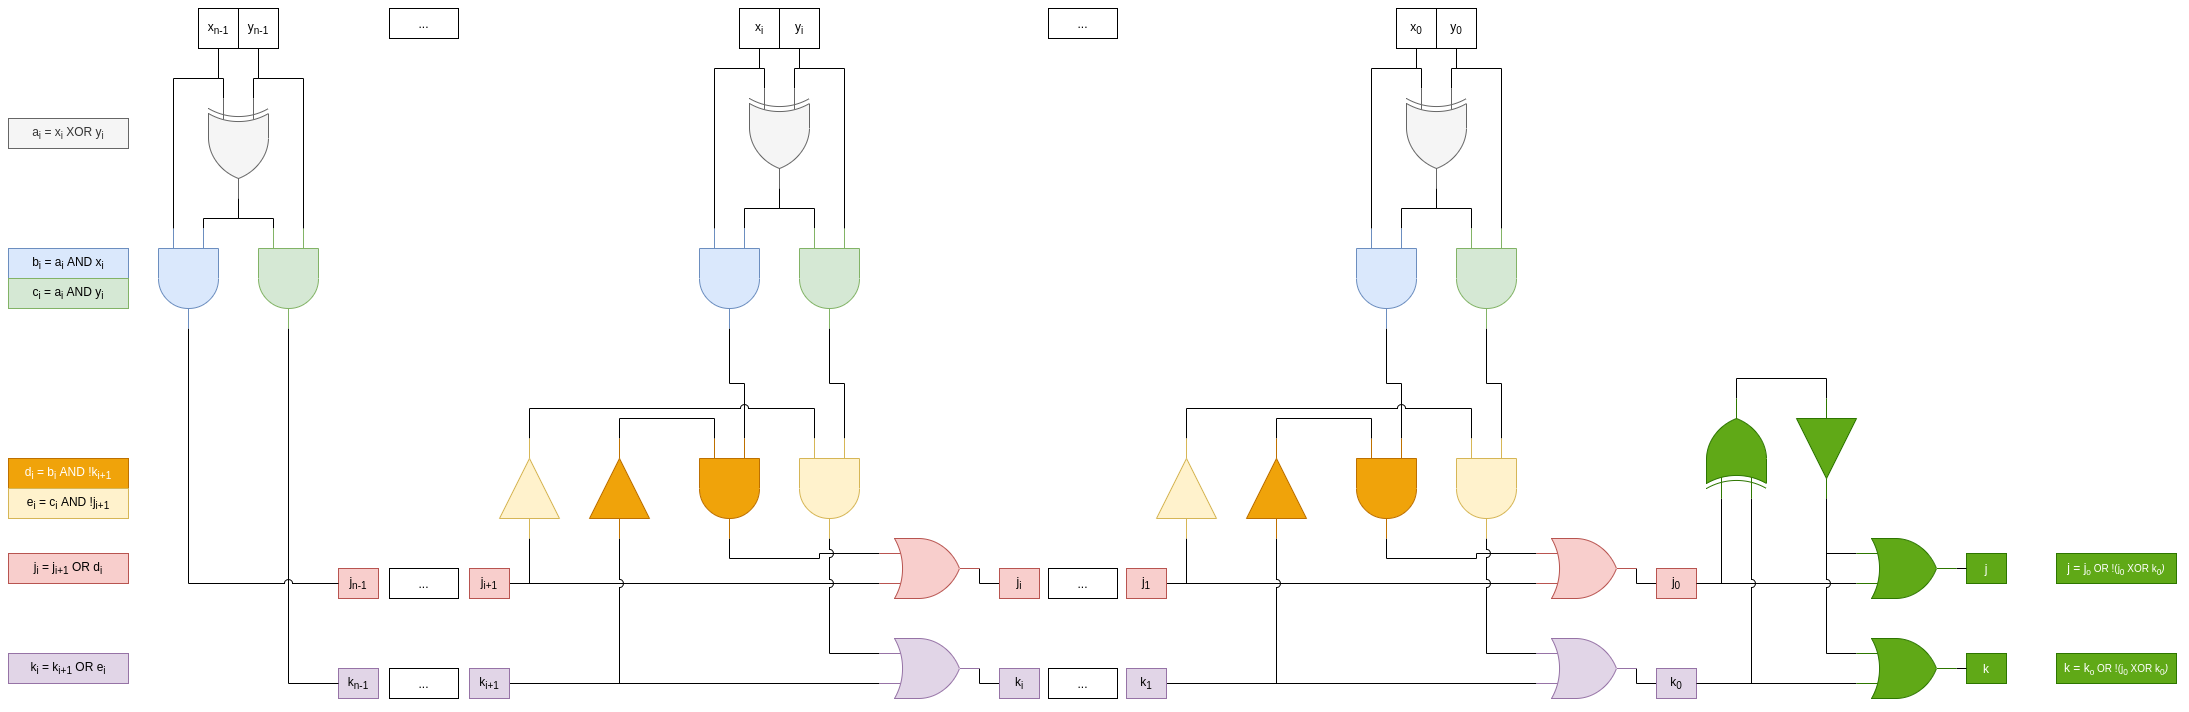
\includegraphics[width=\textwidth]{1_circuit}
		\caption{bigger(x, y) circuit)}
		\label{fig:circuit}
\end{figure}


\section{Homomorphic encryption}

\subsection{Textbook ElGamal}

Let $\oplus$, $\otimes$ be the multiplication operation in $\mathbb{G}$. Let
$m_1, m_2$ be two plaintexts. Let $y$ be the El Gamal public key. Then:

\begin{align*}
		Enc(y, m_1) & = (g^{r_1}, m_1 \cdot y^{r_1}) \\
		Enc(y, m_2) & = (g^{r_2}, m_2 \cdot y^{r_1})
\end{align*}

And:
\begin{align*}
		Enc(y, m_1) \otimes Enc(y, m_2) & = (g^{r_1} \otimes g^{r_2}, m_1 \cdot y^{r_1} \otimes m_2 \cdot y^{r_2}) \\
										& = (g^{r_1 + r_2}, (m_1 \cdot m_2) y^{r_1 + r_2}) \\
										& = Enc(y, m_1 \oplus m_2)\ \text{for}\ r := r_1 + r_2
\end{align*}

\subsection{Textbook RSA}

Let $\oplus$, $\otimes$ be the multiplication operation in $\mathbb{Z}_N^{*}$.
Let $m_1, m_2$ be two plaintexts. Let $(N, e)$ be the RSA public key. Then:

\begin{align*}
		Enc((N, e), m_1) \otimes Enc((N, e), m_2) & = (m_1^e \mod N) \otimes (m_2^e \mod N) \\
												  & = (m_1 \cdot m_2)^e \mod N \\
												  & = Enc((N, e) m_1 \oplus m_2)
\end{align*}

\end{document}
